\section{Трансформационный моноид} % ClassCard %ClassLength
\begin{frame}{Основные свойства трансформационного моноида}
    \vspace*{-6pt}
    \begin{block}{\bf Определение}
        Трансформационный моноид $\mathcal{M}_{\Aut}$ для ДКА $\Aut$ --- это моноид функций $F_{\xi}$ таких, что $F_{\xi}(q_i)= q_j\iff (q_i\transit{\xi} q_j$ в $\Aut)$. Иначе можно сказать, что трансформационный моноид $\mathcal{M}_{\Aut}$ определяется множеством классов эквивалентности
        $\bigl\{w\mid w\in\Sigma^+\bigr\}$ таким, что $w_i = w_j\iff F_{w_i}=F_{w_j}$.
    \end{block} % descriptive documentation 
    \begin{itemize}
        \item $\mathcal{M}_{\Aut}$ определяется фактормножеством классов эквивалентности и правилами переписывания, задающими эквивалентность. $\empt$ обычно не включается в множество $w_i$.
        \item Поскольку множество функций $F_{w_i}$ в случае ДКА конечно, то $\mathcal{M}_{\Aut}$ содержит конечное число классов эквивалентности (верно и обратное: каждый такой моноид определяет некоторый ДКА).
        \item Трансмоноид строится для ДКА без ловушек; переход в ловушку обозначается в таблице переходов просто прочерком.
        \item Для единообразия записи трансформаций и перестановок в алгебре, в таблице переходов пишут только номера состояний $\Aut$.
    \end{itemize} % overall documentation
\end{frame}

\begin{frame}{Построение трансформационного моноида}
    \begin{center}
        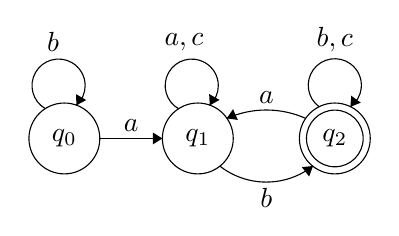
\begin{tikzpicture}[scale=0.15] % the initial automaton placeholder
            \tikzstyle{every node}+=[inner sep=0pt]
            \draw [black] (24.9,-17.8) circle (3);
            \draw (24.9,-17.8) node {$q_0$};
            \draw [black] (36.2,-17.8) circle (3);
            \draw (36.2,-17.8) node {$q_1$};
            \draw [black] (47.8,-17.8) circle (3);
            \draw (47.8,-17.8) node {$q_2$};
            \draw [black] (47.8,-17.8) circle (2.4);
            \draw [black] (27.9,-17.8) -- (33.2,-17.8);
            \fill [black] (33.2,-17.8) -- (32.4,-17.3) -- (32.4,-18.3);
            \draw (30.55,-17.3) node [above] {$a$};
            \draw [black] (23.294,-15.28) arc (240.24286:-47.75714:2.25);
            \draw (23.94,-10.5) node [above] {$b$};
            \fill [black] (25.92,-14.99) -- (26.75,-14.55) -- (25.89,-14.05);
            \draw [black] (34.58,-15.289) arc (240.57068:-47.42932:2.25);
            \draw (35.03,-10.45) node [above] {$a,c$};
            \fill [black] (37.21,-14.99) -- (38.04,-14.54) -- (37.16,-14.04);
            \draw [black] (45.951,-20.128) arc (-51.88249:-128.11751:6.401);
            \fill [black] (45.95,-20.13) -- (45.01,-20.23) -- (45.63,-21.02);
            \draw (42,-21.99) node [below] {$b$};
            \draw [black] (46.477,-15.12) arc (234:-54:2.25);
            \draw (47.8,-10.55) node [above] {$b,c$};
            \fill [black] (49.12,-15.12) -- (50,-14.77) -- (49.19,-14.18);
            \draw [black] (38.655,-16.105) arc (114.1229:65.8771:8.185);
            \fill [black] (38.65,-16.1) -- (39.59,-16.23) -- (39.18,-15.32);
            \draw (42,-14.89) node [above] {$a$};
        \end{tikzpicture}
    \end{center}
    \only<1>{Oпределим соответствие между буквами и множествами переходов по ним и будем расширять этот список новыми словами в лексикографическом порядке. Если очередное слово задаёт такую же трансформацию, как и уже рассмотренное, порождаем соответствующее правило переписывания.}%overall documentation

    \begin{center}
        \begin{tabular}{c||c}\hline
            \cellcolor{blue!10}\textbf{Классы эквивалентности} & \cellcolor{blue!10}\textbf{Правила переписывания} \\\hline\hline
            \smallskip
            $\begin{array}{r|ccc} % the equivalence class table placeholder
                        & 0 & 1 & 2          \\\hline
                     a  & 1 & 1 & 1          \\
                     b  & 0 & 2 & 2          \\
                     c  & - & 1 & 2\only<2>{ \\
                     ab & 2 & 2 & 2          \\
                     bc & - & 2 & 2          \\
                     ca & - & 1 & 1
                     }
                 \end{array}$
                                                               &
            \only<2>{$\begin{array}{cc} % the rewrite rule table placeholder
                                  aa\to a   & ac\to a   \\
                                  ba \to a  & bb\to b   \\
                                  cb\to bc  & cc\to c   \\
                                  abc\to ab & bca\to ca \\
                                  cab\to bc
                              \end{array}$}
        \end{tabular}
    \end{center}
    Всего классов эквивалентности: $6$ % the ClassCard placeholder

    Максимальная длина факторслова в классах эквивалентности: $2$ % the ClassLength placeholder 
\end{frame}